\documentclass[12pt]{article}

\usepackage{latexsym}
\usepackage{amsfonts}
\usepackage{amsmath, amsthm, amssymb}
\usepackage{graphicx}
\usepackage{hyperref}

\setlength{\textheight}{10in}
\setlength{\textwidth}{6.5in}
\setlength{\topmargin}{-1.0in}
\setlength{\parskip}{0.15in}
\setlength{\oddsidemargin}{-0.1in}

\newcommand{\DS} [1] {${\displaystyle #1}$}

\author{Michael Walker}
\title{Math 2311 $-$ Assignment 1}
\date{\today}

\begin{document}
\maketitle
\begin{enumerate}
        \item
              Determine if each of the following sets is a vector space.
              \begin{enumerate}
                      \item $V=$\DS{ \left\{ \left[ \begin{array}{c}
                                                    x \\
                                                    y
                                            \end{array} \right] \in\mathbb{R}^2 \ | \ x \geq{y} \right\}}
                            with the usual scalar multiplication
                            and vector addition from $\mathbb{R}^2$
              \end{enumerate}
              \paragraph{Answer:} No, $V$ is not a vector space.
              \begin{proof}
                      let $({x_0}, {y_0}), ({x_1}, {y_1}) \in V$,
                      and take the vector space operations on $V$
                      to be the usual operations of $vector$
                      addition and $scalar$ multiplication; that is,
                      \begin{align}
                              ({x_0}, {y_0})+ & ({x_1}, {y_1}) =({x_0}+{x_1}, {y_0}+{y_1}) \\
                                              & k({x_0}, {y_0}) = ({kx_0}, {ky_0})
                      \end{align}
                      $V$ is closed under scalar addition since ${x_0 + x_1} \ge {y_0 + y_1}$ \\\\
                      However, by properties of inequalities if the constant,
                      k, is negative, we must reverse the symbol to preserve the inequality relation.

                      Given that k is negative, ${x\geq y} \rightarrow {kx\leq ky}$
              \end{proof}
              \pagebreak
              \begin{enumerate}
                      \item[(b)] Consider the set $W = \{f \in F(-\infty, \infty) \ | f(1) = 0\}$
                            with the usual scalar multiplication and vector addition from
                            $F(-\infty, \infty)$.
                            Is $W$ a vector space?
              \end{enumerate}
              \paragraph{Answer:} Yes, $W$ is a vector space.
              \begin{proof}
                      Since we know that $F(-\infty, \infty)$ (with the usual operations) is a vector space,
                      and since $W$ is a subset of $F(-\infty, \infty)$ (with the same operations),
                      it suffices to prove that $W$ is a subspace of $F(-\infty, \infty)$.
                      To this end we must show three things:
                      \begin{enumerate}
                              \item That $W$ is non-empty.
                              \item That $W$ is closed under addition.
                              \item That $W$ is closed under scalar multiplication.
                      \end{enumerate}
                      There exists a function $\mathbf{0}$ in $F(-\infty, \infty)$
                      defined by $\mathbf{0}(x)=0$ for all $x$.
                      Clearly $\mathbf{0}(1)=f(1)=0$ so $W$ is non-empty.

                      Now suppose $f$ and $g$ are two functions in $W$. We must show that $f+g$ is in $W$.
                      \begin{align*}
                              (f+g)(1) & = f(1) + g(1) & \textrm{(definition of addition of functions)} \\
                                       & = 0           & \textrm{($f$ and $g$ are in $W$)}
                      \end{align*}
                      Finally, to show that $W$ is closed under scalar multiplication,
                      suppose $f$ is in $W$ and $k$ is a scalar, then
                      \begin{align*}
                              (kf)(1) & = kf(1) & \textrm{(definition of scalar multiplication on functions)} \\
                                      & = 0     & \textrm{($f$ is in $W$)}
                      \end{align*}
                      so $(kf)$ is in $W$ and $W$ is closed under scalar multiplication.

                      Therefore $W$ is a subspace of $F(-\infty, \infty)$ and hence is a vector space.
              \end{proof}
              \pagebreak
        \item
              Let $V$ be a vector space.
              \begin{enumerate}
                      \item If $k$ is any scalar, prove that $k\vec{0} = \vec{0}$.
              \end{enumerate}
              \begin{proof}
                      \begin{align*}
                              k(\vec{0} + \vec{0})   & = k\vec{0} + k\vec{0}                 & \textrm{(vector space axiom 7)} \\
                              k\vec{0}               & = k\vec{0} + k\vec{0}                 & \textrm{(vector space axiom 4)} \\
                              k\vec{0} + (-k\vec{0}) & = (-k\vec{0}) + (k\vec{0} + k\vec{0}) & \textrm{(vector space axiom 5)} \\
                              k\vec{0} + (-k\vec{0}) & = ((-k\vec{0}) + k\vec{0}) + k\vec{0} & \textrm{(vector space axiom 3)} \\
                              \vec{0}                & = \vec{0} + k\vec{0}                  & \textrm{(vector space axiom 5)} \\
                                                     & = k\vec{0}                            & \textrm{(vector space axiom 4)}
                      \end{align*}
              \end{proof}
              \begin{enumerate}
                      \item[(b)] Prove that the zero vector in $V$ is unique.
              \end{enumerate}
              \begin{proof}
                      We must show that there is only one vector, $\vec{0}$, with the property that \\
                      $\vec{0} + \vec{v} = \vec{v} + \vec{0} = \vec{v}$.

                      Suppose $\vec{0_1}$ and $\vec{0}$ are zero vectors in $V$ Then
                      \begin{align*}
                              \vec{0_1} & = \vec{0_1} + \vec{0} & \textrm{(vector space axiom 4)} \\
                                        & = \vec{0} + \vec{0_1} & \textrm{(vector space axiom 2)} \\
                                        & = \vec{0}             & \textrm{(vector space axiom 4)}
                      \end{align*}
                      Therefore $\vec{0_1} = \vec{0}$. So, the zero vector is unique.
              \end{proof}
        \item Determine if each of the following are subspaces of $M_{nn}$
              \begin{enumerate}
                      \item \DS{ \left\{A\in{M_{nn}} \ | det (A) = 0 \right\}}
                            \paragraph{Answer:} No, ${ \left\{A \in M_{nn} \
                                                    | \det (A) = 0 \right\}}$ is not a subspace of $M_{nn}$.
                            \begin{proof}
                                    \begin{equation*}
                                            \det
                                            \begin{vmatrix}
                                                    {1} & {0} \\
                                                    {0} & {0} \\
                                            \end{vmatrix}
                                            {= 0},
                                            \det
                                            \begin{vmatrix}
                                                    {0} & {0} \\
                                                    {0} & {1} \\
                                            \end{vmatrix}
                                            = 0
                                    \end{equation*}
                                    \begin{equation*}
                                            \begin{bmatrix}
                                                    {1} & {0} \\
                                                    {0} & {0} \\
                                            \end{bmatrix}
                                            +
                                            \begin{bmatrix}
                                                    {0} & {0} \\
                                                    {0} & {1} \\
                                            \end{bmatrix}
                                            =
                                            \begin{bmatrix}
                                                    {1} & {0} \\
                                                    {0} & {1} \\
                                            \end{bmatrix}
                                    \end{equation*}
                                    \begin{equation*}
                                            \det
                                            \begin{vmatrix}
                                                    {1} & {0} \\
                                                    {0} & {1} \\
                                            \end{vmatrix}
                                            = 1 \neq 0
                                    \end{equation*}
                            \end{proof}\pagebreak
                      \item \DS{ \left\{A \in{M_{nn}} \ | tr (A) = 0 \right\}}
                            \paragraph{Answer:} Yes, $W={ \left\{A \in M_{nn} \ |
                                    tr(A) = 0 \right\}}$ is a subspace of $M_{nn}$.
                            \begin{proof}
                                    Let [$B = ({b_{ii}})]\in W$ be a square matrix of order n such that $tr(B)=0$ and let ${k}$ be any scalar.\\\\
                                    The set $W$ is non empty because if we let ${a_{ii}=0}$
                                    for all i then $tr(A)=0$ therefore $W$ contains the $\mathbf{0}$ matrices.
                                    It remains to show that W is closed under addition and scalar multiplication.
                                    \begin{align*}
                                            addition:       &                                                   \\
                                            tr(A+B)         & = \sum_{i = 1}^{n}(a_{ii}+b_{ii})                 \\
                                                            & = \sum_{i = 1}^{n}a_{ii} + \sum_{i = 1}^{n}b_{ii} \\
                                                            & = tr(A) + tr(B)                                   \\
                                                            & = 0 + 0                                           \\
                                                            & = 0                                               \\
                                            multiplication: &                                                   \\
                                            tr(kA)          & = \sum_{i = 1}^{n}(k\cdot a_{ii})                 \\
                                                            & = k\cdot \sum_{i = 1}^{n}a_{ii}                   \\
                                                            & = k\cdot tr(A)                                    \\
                                                            & = k\cdot 0                                        \\
                                                            & = 0
                                    \end{align*}
                                    To be clear, if we take some $C = A+B$ such that A and B are in $W$,
                                    then for all $C = (c_{ii})$, the sum will be $0$, so $C$ is also in $W$.
                                    Therefore $W$ is a subspace of $M_{nn}$.
                            \end{proof}
                            \pagebreak
                      \item \DS{ \left\{A \in{M_{nn}} \ | A^T = A \right\}}
                            \paragraph{Answer:} Yes, $W={ \left\{A \in{M_{nn}} \ |
                                    A^T = A \right\}}$ is a subspace of $M_{nn}$.
                            \begin{proof}
                                    Let $[B = (b_{ij})]\in W$ be a square matrix of order $n$
                                    such that $b_{ij} = b_{ji}$, and let ${k}$ be any scalar.\\\\
                                    The set $W$ is non empty because, if we let $[A=({a_{ij})]=0}$
                                    for all $(i,j)$ then $W$ contains the $\mathbf{0}$ matrices.
                                    It remains to show that $W$ is closed under addition and scalar multiplication.
                                    \begin{align*}
                                            addition:       &                \\
                                            C               & = (A+B)^T      \\
                                                            & = A^T+B^T      \\
                                                            & = A + B        \\
                                            multiplication: &                \\
                                            (k\cdot A)^{T}  & = k\cdot A^{T} \\
                                                            & = k\cdot A
                                    \end{align*}
                                    so $W$ is a subspace of $M_{nn}$.
                            \end{proof} \pagebreak
              \end{enumerate}

        \item Consider the following vectors in $P_2$: $p_1 = 2 + x + 4x^2$, $p_2 = 1 - x + 3x^2$, $p_3 = 3 + 2x + 5x^2$.
              \begin{enumerate}
                      \item Express the vector $g = 6 + 11x + 6x^2$ as a linear combination of $p_1,p_2,p_3$.
                            \paragraph{Answer: Yes, $(p_1,p_2,p_3)$ = (4, -5, 1)}
                            \begin{proof}
                                    \begin{align*}
                                            (6 + 11x + 6x^2) & =  k_{0}(2 + x + 4x^2) +  k_{1}(1 - x + 3x^2) +  k_{2}(3 + 2x + 5x^2)                                \\
                                                             & =  (k_{0}2 + k_{1} + k_{2}3)  +  (k_{0}x - k_{1}x + k_{2}2x)  +  (k_{0}4x^2 + k_{1}3x^2 + k_{2}5x^2) \\
                                                             & =  (k_{0}2 + k_{1} + k_{2}3)  +  (k_{0} - k_{1} + k_{2}2)x    +  (k_{0}4 + k_{1}3 + k_{2}5)x^2
                                    \end{align*}
                                    \begin{align*}
                                             &
                                            \begin{bmatrix}
                                                    2 & 1  & 3 & \bigm| & 6  \\
                                                    1 & -1 & 2 & \bigm| & 11 \\
                                                    4 & 3  & 5 & \bigm| & 6  \\
                                            \end{bmatrix} \\
                                            [-2r2+r1] \wedge [-4r2+r1]
                                             &
                                            \begin{bmatrix}
                                                    0 & 3  & -1 & \bigm| & -16 \\
                                                    1 & -1 & 2  & \bigm| & 11  \\
                                                    0 & 7  & -3 & \bigm| & -38 \\
                                            \end{bmatrix} \\
                                            r2\leftrightarrow r1
                                             &
                                            \begin{bmatrix}
                                                    1 & -1 & 2  & \bigm| & 11  \\
                                                    0 & 3  & -1 & \bigm| & -16 \\
                                                    0 & 7  & -3 & \bigm| & -38 \\
                                            \end{bmatrix} \\
                                            \frac{1}{3}r2
                                             &
                                            \begin{bmatrix}
                                                    1 & -1 & 2            & \bigm| & 11            \\
                                                    0 & 1  & \frac{-1}{3} & \bigm| & \frac{-16}{3} \\
                                                    0 & 7  & -3           & \bigm| & -38           \\
                                            \end{bmatrix} \\
                                            -7r2+r3
                                             &
                                            \begin{bmatrix}
                                                    1 & -1 & 2            & \bigm| & 11            \\
                                                    0 & 1  & \frac{-1}{3} & \bigm| & \frac{-16}{3} \\
                                                    0 & 0  & \frac{-2}{3} & \bigm| & \frac{-2}{3}  \\
                                            \end{bmatrix} \\
                                    \end{align*}
                                    \begin{align*}
                                            -\frac{3}{2}r3
                                             &
                                            \begin{bmatrix}
                                                    1 & -1 & 2            & \bigm| & 11            \\
                                                    0 & 1  & \frac{-1}{3} & \bigm| & \frac{-16}{3} \\
                                                    0 & 0  & 1            & \bigm| & 1             \\
                                            \end{bmatrix} \\
                                            \frac{1}{3}r3+r2
                                             &
                                            \begin{bmatrix}
                                                    1 & -1 & 2 & \bigm| & 11 \\
                                                    0 & 1  & 0 & \bigm| & -5 \\
                                                    0 & 0  & 1 & \bigm| & 1  \\
                                            \end{bmatrix} \\
                                            r1 + r2
                                             &
                                            \begin{bmatrix}
                                                    1 & 0 & 2 & \bigm| & 6  \\
                                                    0 & 1 & 0 & \bigm| & -5 \\
                                                    0 & 0 & 1 & \bigm| & 1  \\
                                            \end{bmatrix} \\
                                            r1 + r3
                                             &
                                            \begin{bmatrix}
                                                    1 & 0 & 0 & \bigm| & 4  \\
                                                    0 & 1 & 0 & \bigm| & -5 \\
                                                    0 & 0 & 1 & \bigm| & 1  \\
                                            \end{bmatrix}
                                    \end{align*}
                                    \begin{equation*}
                                            \therefore (k_{1}, k_{2}, k_{3}) = (4, -5, 1) \\
                                    \end{equation*}
                            \end{proof}
                            \pagebreak
                      \item Does $\{p_1,p_2,p_3\}$ span $P_2$?
                            \paragraph{Answer: Yes, $span(\{\vec{p_{1}},\vec{p_{2}},\vec{p_{3}}\}) = P_{2}$}
                            \begin{proof}
                                    An arbitrary vector in $P_{2}$ is of the form $\vec{p}=a+bx+cx^2$ and so becomes,\\\\
                                    $k_{0}(2 + x + 4x^2) +  k_{1}(1 - x + 3x^2) + k_{2}(3 + 2x + 5x^2) = a+bx+cx^2$\\\\
                                    which we can rewrite as \\\\
                                    $(k_{0}2 + k_{1} + k_{2}3) + (k_{0} - k_{1} + k_{2}2)x + (k_{0}4 + k_{1}3 + k_{2}5)x^2 = a+bx+cx^2$\\\\
                                    Equating corresponding coefficients yields a linear system whose augmented matrix is
                                    \begin{align*}
                                            A =
                                            \begin{bmatrix}
                                                    2 & 1  & 3 & \bigm| & a \\
                                                    1 & -1 & 2 & \bigm| & b \\
                                                    4 & 3  & 5 & \bigm| & c \\
                                            \end{bmatrix}
                                    \end{align*}
                                    Our problem reduces to ascertaining whether this system is consistent for
                                    all values of a, b, and c. This can be determined if its coefficient matrix
                                    has a nonzero determinant, from our theorem for equivalent statements.
                                    If $A$ is an $n$ $x$ $n$ matrix such that $\det(A)\neq0$ then $A\vec{x}=\vec{0}.$\\\\
                                    It follows from solution (a) that
                                    \begin{align*}
                                            \begin{bmatrix}
                                                    2 & 1  & 3 & \bigm| & 0 \\
                                                    1 & -1 & 2 & \bigm| & 0 \\
                                                    4 & 3  & 5 & \bigm| & 0 \\
                                            \end{bmatrix}
                                            =
                                            \begin{bmatrix}
                                                    1 & 0 & 0 & \bigm| & 0 \\
                                                    0 & 1 & 0 & \bigm| & 0 \\
                                                    0 & 0 & 1 & \bigm| & 0 \\
                                            \end{bmatrix}
                                    \end{align*}
                                    so $A$ is consistent for every choice $a,b,$ and $c$.
                                    Thus, the vectors in $\{\vec{p_{1}},\vec{p_{2}},\vec{p_{3}}\}$ span $P_{2}$.
                            \end{proof}
                      \item Is $\{p_1,p_2,p_3\}$ linearly independent?
                            \paragraph{Answer: Yes, $k_{1}\vec{p1} + k_{2}\vec{p2} + k_{3}\vec{p3} = \vec{0}$}
                            \begin{proof}
                                    From part (b) we have                                     \begin{align*}
                                            \begin{bmatrix}
                                                    2 & 1  & 3 & \bigm| & 0 \\
                                                    1 & -1 & 2 & \bigm| & 0 \\
                                                    4 & 3  & 5 & \bigm| & 0 \\
                                            \end{bmatrix}
                                            =
                                            \begin{bmatrix}
                                                    1 & 0 & 0 & \bigm| & 0 \\
                                                    0 & 1 & 0 & \bigm| & 0 \\
                                                    0 & 0 & 1 & \bigm| & 0 \\
                                            \end{bmatrix}
                                    \end{align*}
                                    Therefore $(k_{1}, k_{2}, k_{3}) = (0,0,0)$ so $\{\vec{p_{1}}, \vec{p_{2}}, \vec{p_{3}}\}$ is linearly independent
                            \end{proof}
                            \pagebreak
              \end{enumerate}
        \item Consider the following planes in $\mathbb{R}^3$. $P_1: 2x + 3y - z = 0$ and $P_2: x + 2y - 2z = 0$
              \begin{enumerate}
                      \item Find a set of vectors that spans $P_1$.
                            \paragraph{Answer: any $2$ vectors from the set $\{(0, 1, 3), (-1, 0, 2), (-3, 2, 0)\}$}
                            \begin{proof}
                                    \begin{align*}
                                            \textrm{Let }\vec{e_1} = (1, 0, 0),\ \vec{e_2} = (0, 1, 0)\ \vec{e_3} = (0, 0, 1)
                                    \end{align*}
                                    be unit vectors in $R^3$, we will compute the cross products
                                    \begin{align*}
                                            \vec{e_1} \times (2, 3, -1),\ \vec{e_2} \times (2, 3, -1),\ \vec{e_3} \times (2, 3, -1)
                                    \end{align*}
                                    to find a set of vectors that spans $P_1$
                                    \begin{align*}
                                            (1,0,0) \times (2,3,-1) & = ( (0)(-1) - (0)(3), (0)(2)-(1)(-1), (1)(3)-(0)(2) ) \\
                                                                    & = (0, 1, 3)                                           \\\\
                                            (0,1,0) \times (2,3,-1) & = ( (1)(-1) - (0)(3), (0)(2)-(0)(-1), (0)(3)-(1)(2) ) \\
                                                                    & = (-1, 0, -2)                                         \\\\
                                            (0,0,1) \times (2,3,-1) & = ( (0)(-1) - (1)(3), (1)(2)-(0)(-1), (0)(3)-(0)(2) ) \\
                                                                    & = (-3, 2, 0)
                                    \end{align*}
                                    any $2$ vectors from the set $\{(0, 1, 3), (-1, 0, 2), (-3, 2, 0)\}$ will span the plane $P_1$.
                            \end{proof}
                      \item Find a set of vectors that spans $P_2$.
                            \paragraph{Answer: any $2$ vectors from the set $\{(0, 2, 2) , (-2, 0, -1), (-2, 1, 0)\}$}
                            \begin{proof}
                                    \begin{align*}
                                            \textrm{Let }\vec{e_1} = (1, 0, 0),\ \vec{e_2} = (0, 1, 0)\ \vec{e_3} = (0, 0, 1)
                                    \end{align*}
                                    be unit vectors in $R^3$, we will compute the cross products
                                    \begin{align*}
                                            \vec{e_1} \times (1, 2, -2),\ \vec{e_2} \times (1, 2, -2),\ \vec{e_3} \times (1, 2, -2)
                                    \end{align*}
                                    to find a set of vectors that spans $P_2$
                                    \begin{align*}
                                            (1,0,0) \times (1, 2, -2) & = ( (0)(-2) - (0)(2), (0)(1)-(1)(-2), (1)(2)-(0)(1) ) \\
                                                                      & = (0, 2, 2)                                           \\\\
                                            (0,1,0) \times (1, 2, -2) & = ( (1)(-2) - (0)(2), (0)(1)-(0)(-2), (0)(3)-(1)(1) ) \\
                                                                      & = (-2, 0, -1)                                         \\\\
                                            (0,0,1) \times (1, 2, -2) & = ( (0)(-2) - (1)(2), (1)(1)-(0)(-2), (0)(3)-(0)(1) ) \\
                                                                      & = (-2, 1, 0)
                                    \end{align*}
                                    any $2$ vectors from the set $\{(0, 2, 2) , (-2, 0, -1), (-2, 1, 0)\}$ will span the plane $P_2$.
                            \end{proof}
                            \pagebreak
                      \item Find a set of vectors that spans the intersection of $P_1$ and $P_2$. (Recall that we showed the intersection of two subspaces is a subspace).
              \end{enumerate}
              \begin{figure}[htbp]
                      \centering
                      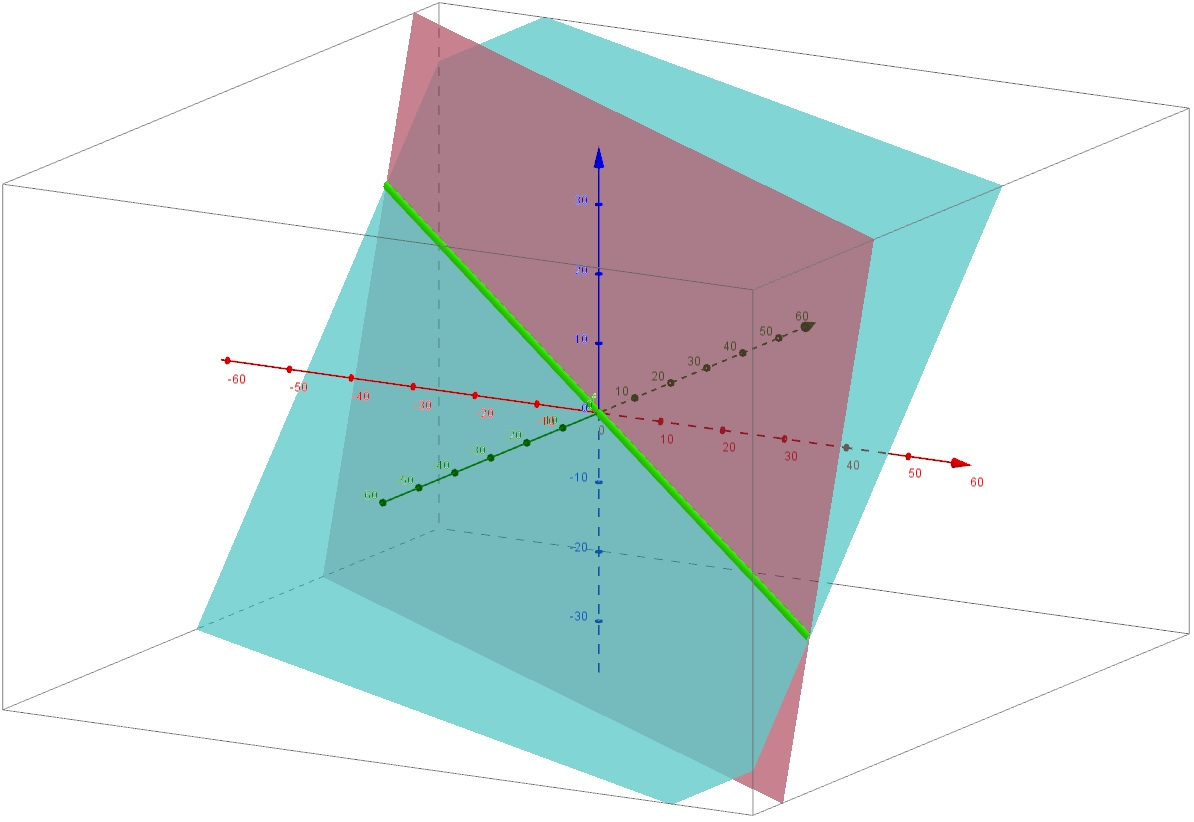
\includegraphics[width = 0.8\textwidth]{//home/the-scientist/linear/linear-algebra/asg1/resources/sol_space_white.jpg}
                      \caption{$p_{1} \bigcap p_{2}$ \url{https://www.geogebra.org/3d/kuawemzp}\label{fig:solution space}}
              \end{figure}
\end{enumerate}
\end{document}
